
\section{Background and Motivation}

\subsection{Convolution Operation}
We use the following notations throughout this paper. We use $I$, $F$ and $O$ to denote an input, a filter and an output tensor
respectively. Each tensor is indexed according to its batch size ($N$), channel ($C$), height ($H$) and width ($W$). For example, $I_N$,
$I_C$, $I_H$ and $I_W$ represent the batch size, number of channels, width and height of an input.

The convolution operation is commonly used to extract various features from the input feature maps via convolutional filters. The computation
in the convolution stage takes a batch of $I_N$ 2D multi-channel feature maps of size $I_C \times I_H \times I_W$ and a bank of $F_N$ 2D
multi-channel filters of size $F_C \times F_H \times F_W$ ($F_C = I_C$) as inputs. The result of convolution is a batch of $O_N$
($O_N=I_N$) 2D multi-channel output feature maps of size $O_C \times O_H \times O_W$ ($O_C=F_N$). To generate one output feature map, all
filters are used to convolve with the same input feature map. Each filter slides over the input feature map and performs an elementwise
multiplication with the part of input where it is currently located  and then sums up the results over all channels.

\begin{figure}
\centering
  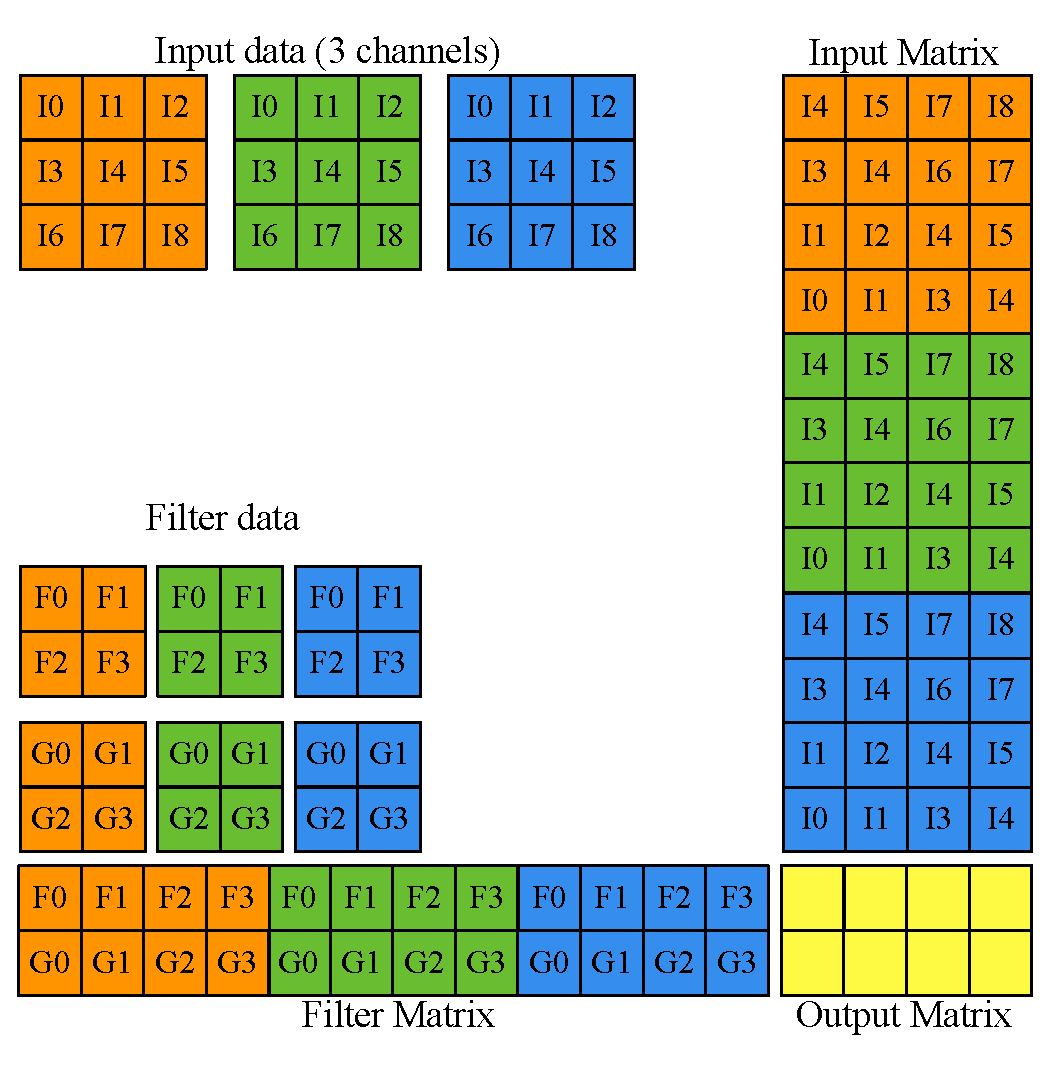
\includegraphics[width=0.75\columnwidth,height=6cm]{./figure/convlowering.eps}
  \caption{An illustration of how to convert a simple convolution into a matrix multiplication. Two filters are used to convolve with a 3-channel input.}
  \label{fig:convlowering}
\end{figure}

Many algorithms, such as FFT-based and Winograd-based convolutions have been utilized to optimize the convolution operation, but they all need to
transform 4D tensors into the desired matrix, thus incurring high memory overhead. Figure \ref{fig:convlowering}, which is taken from
\cite{ChetlurWVCTCS14}, illustrates how to convert a simple convolution into a matrix multiplication. Numerous duplicate elements, which can increase the memory overhead and offset some performance gains caused by the reduction in computation complexity, are present in the input matrix.


\subsection{Motivation Example}

As a motivation, consider Figure \ref{fig:twostrategies} that shows a simple 2D convolution executing on a GPU. Here, we slide a $5 \times
5$ filter over a $6 \times 11$ image to produce a $2 \times 7$ output. Each thread calculates one column of the output. Threads 0 and 1
demonstrate the process of sliding the filter along the width dimension. Both threads load two overlapped regions from the input image,
thereby generating four duplicate columns. Thread 6 demonstrates the process of sliding the filter along the height dimension; it loads two
overlapped regions and generates four duplicate rows.

Our optimization algorithms can eliminate two types of duplication and thus reduce the number of memory transactions. In the proposed column reuse algorithm, we let each thread load the necessary first and last columns and retrieve the remaining from other threads through shuffle
instructions. The difference in the usage of shuffle instructions between our algorithms and the previous study
\cite{vasilache2014fast} is discussed in Section \ref{sec:strategies}. In the proposed row reuse algorithm, we let each thread load overlapped
rows only once and multiply each row with multiple rows of a filter to calculate multiple output elements. A major performance issue
encountered in our implementation is that the thread local arrays with dynamic indexing are placed in the local memory, which possesses the same
access latency as the global memory. To solve this problem, we use pack and unpack operations to transform dynamic indexing into static indexing.

\begin{figure}
\centering
  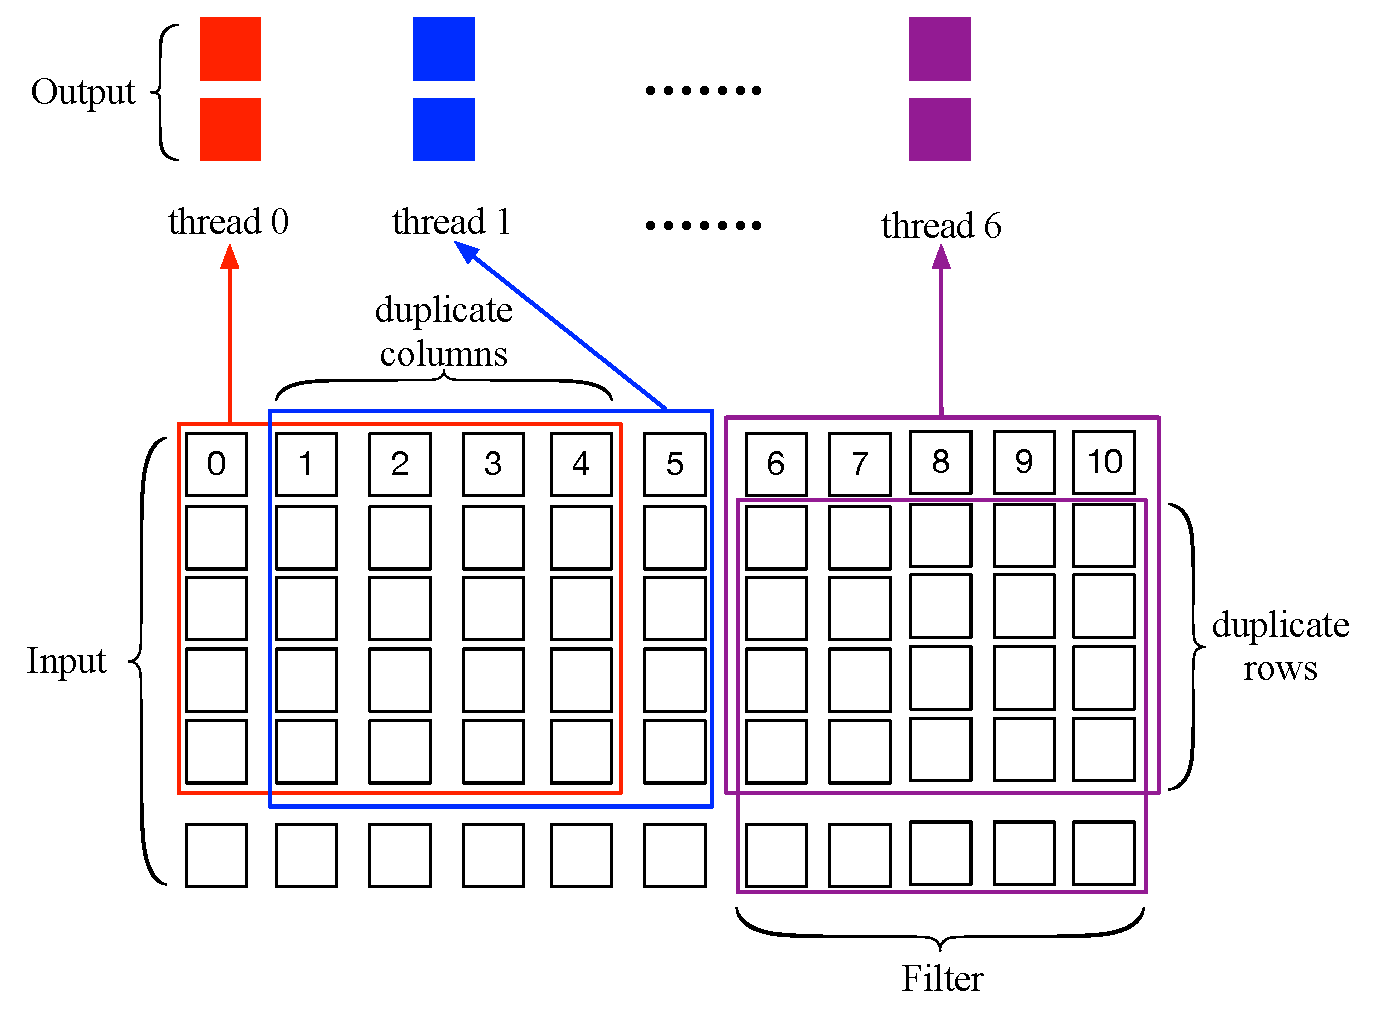
\includegraphics[width=\columnwidth,height=6cm]{./figure/twostrategies.eps}
  \caption{An illustration of how to perform 2D convolution on GPU. Filter size is $5 \times 5$, input image size is $6 \times 11$ and output size is $2 \times 7$. Each thread calculates one column of the output. Threads 0 and 1 load needed regions from input image with four duplicate columns. Thread 6 loads two overlapped regions from input image and generates four duplicate rows. Numbers in the square denote the index of input elements.}
  \label{fig:twostrategies}
\end{figure}
